\section{The crossing of every bin}\label{sec:allbin}

The same question makes sense for each bin: at which $p$ is bin $k$ exactly
as likely as an endpoint? Figure~\ref{fig:allbin} shows the answer for 3
values of $N$. The crossing $1-p_{a,N-a}$ decreases as the bin moves in from
the edge, from order $N^{-1/2}$ next to the edge to order $(\log N)/N$ in the
middle. This section proves this picture.

\subsection{Ordering the crossings}\label{sec:allbin-order}

Let $a,b\ge1$ be integers, $N=a+b$ and $p>0$, and recall that
$S_{a,b}(u)=P_N(a)/P_N(0)$ with $u=(1-p)/p$. Theorem~\ref{thm:pmf} and
$\binom{m-1}{r+1}=\frac{m-1-r}{r+1}\binom{m-1}{r}$ for $m=a,b$ give
\begin{equation}\label{eq:allbin-polynomial}
 S_{a,b}(u)=\sum_{r\ge0}\binom{a-1}{r}\binom{b-1}{r}
 \Bigl(2u^{2r+1}+\frac{N-2-2r}{r+1}u^{2r+2}\Bigr).
\end{equation}
Its coefficients are nonnegative, as $N-2-2r\ge|b-a|$ for $r<\min(a,b)$, and
the linear one is $2$. So there is a unique $u_{a,b}>0$ with
$S_{a,b}(u_{a,b})=1$, and $p_{a,b}=1/(1+u_{a,b})$. As $S_{a,b}(u)\ge2u$, we
have $u_{a,b}\le\frac12$ and $p_{a,b}\in[\frac23,1)$, with $p_{a,b}=\frac23$
only for $a=b=1$.

\begin{proposition}[ordering the crossings]\label{prop:allbin-order}
If $a<b-1$, then
\[
 u_{a+1,b-1}<u_{a,b},\qquad p_{a+1,b-1}>p_{a,b}.
\]
Also $p_{a,b+1}>p_{a,b}$ for all positive $a,b$. In fact the corresponding
inequalities between the polynomials $S_{a+1,b-1}$ and $S_{a,b}$, or
$S_{a,b+1}$ and $S_{a,b}$, hold coefficientwise, with at least one strict
coefficient.
\end{proposition}

In words: a bin closer to the middle, or in a longer row, needs a larger $p$
to fall to the endpoint height.

\begin{proof}
For fixed $N$ and $r\le a-1$,
$\binom{a-1}{r}\binom{b-1}{r}=(r!)^{-2}\prod_{j=0}^{r-1}(a-1-j)(b-1-j)$, a
product of positive factors. Each factor grows when $(a,b)$ becomes
$(a+1,b-1)$, by $(a-j)(b-2-j)-(a-1-j)(b-1-j)=b-a-1>0$. The even multiplier
$(N-2-2r)/(r+1)$ is unchanged, and it is nonnegative where either product is
nonzero, since then $r\le a$ and $N-2-2r\ge b-a-2\ge0$. New summands are
nonnegative, and the cubic coefficient grows strictly, from $2(a-1)(b-1)$ to
$2a(b-2)$. Increasing $b$ with $a$ fixed increases the binomial coefficients
of Theorem~\ref{thm:pmf}, and the quadratic coefficient $N-2$ strictly. A
polynomial with nonnegative coefficients that dominates another
coefficientwise, strictly somewhere, is strictly larger at every $u>0$, so its
root is smaller.
\end{proof}

The ordering of the bin heights below also follows from the interior
log-concavity of Dekking and Kong~\cite[Proposition~4.3]{dekkingkong2011}. We
use the coefficients because they also give the strict gap in the next
proposition.

\begin{proposition}[adjacent bins and global extrema]\label{prop:adjacent}
For $N\ge2$ and $0<p<1$, an adjacent bin has the same probability as an
endpoint precisely at
\[
p_N^{\mathrm{adj}}=\frac{1+\sqrt{N-1}}{2+\sqrt{N-1}}.
\]
For $0<p<1$, the endpoints are the least likely bins if
$p<p_N^{\mathrm{adj}}$, bins $1$ and $N-1$ are if $p>p_N^{\mathrm{adj}}$, and
they tie at equality. For $N\ge4$, the central crossing satisfies
$p_N>p_N^{\mathrm{adj}}$. At $p=p_N$, the middle and endpoints attain the
global maximum and bins $1,N-1$ attain the global minimum. For $N=2,3$,
$p_N=p_N^{\mathrm{adj}}$ and every bin ties at the crossing.
\end{proposition}

So at the central crossing the row has the shape of a W: high at the 2 ends
and in the middle, and lowest next to the ends.

\begin{proof}
By \eqref{eq:allbin-polynomial}, $S_{1,N-1}(u)=2u+(N-2)u^2$, with positive
root $u^{\mathrm{adj}}=1/(1+\sqrt{N-1})$. This gives $p_N^{\mathrm{adj}}$ and
the sign change. For $0<p<1$ we have $P_N(k)=P_N(0)S_{k,N-k}(u)$ with
$P_N(0)>0$, so if $1\le k<N-k-1$ Proposition~\ref{prop:allbin-order} gives
$P_N(k)<P_N(k+1)$. By symmetry the middle is the largest interior bin and bins
$1,N-1$ are the smallest, which gives the claims about the least likely bins.
For $N\ge4$ the cubic coefficient $2(\lfloor N/2\rfloor-1)(\lceil N/2\rceil-1)$
of $S_N$ is positive, so $2u_N+(N-2)u_N^2<S_N(u_N)=1$, hence
$u_N<u^{\mathrm{adj}}$ and $p_N>p_N^{\mathrm{adj}}$. At $p_N$ the middle ties
with the endpoints, which gives the global maximum, and bins $1,N-1$ are below
the endpoints, which gives the global minimum. For $N=2,3$ we have
$S_N=S_{1,N-1}$, and symmetry gives the ties.
\end{proof}

So $1-p_N^{\mathrm{adj}}\sim N^{-1/2}$, much larger than
$1-p_N\sim(\log N)/N$. The reason is simple. Away from the ends the single
$\sR$ of bin $1$ needs 2 switches, so $S_{1,N-1}\approx Nu^2$ reaches $1$ only
at $u\approx N^{-1/2}$. (At $p=0$ and $p=1$ there are also ties between bins of
probability $0$.)

\subsection{A Bessel estimate uniform in the bin}\label{sec:allbin-bessel}

Bin $a$ has about $(a^r/r!)(b^r/r!)$ words with $r$ runs of each letter, each
of weight about $u^{2r}$. The sum depends only on $abu^2$, so a bin near the
edge acts like the middle of a shorter row with $\sqrt{ab}$ in place of $N/2$.
Put
\[
 s=\sqrt{ab},\quad A=\frac{ab}{a+b},\quad
 c=\frac{a+b}{2\sqrt{ab}},\quad
 \eta=\frac1c,\quad x=su,\quad J_c(x)=I_0(2x)+cI_1(2x),
\]
and $\widehat S_{a,b}(u)=2uJ_c(su)$. Here $c\ge1$ and $0<\eta\le1$, with
$\eta=1$ exactly when $a=b$.

\begin{theorem}[uniform estimate for every bin]\label{thm:allbin-bessel}
For all positive integers $a,b$ and all $u>0$,
\begin{equation}\label{eq:allbin-bessel}
 0\le 1-\frac{S_{a,b}(u)}{\widehat S_{a,b}(u)}
 \le \frac{(a+b)u^2}{2}+u
 =\frac{x^2}{2A}+\frac xs.
\end{equation}
In particular, for fixed $N$ and $u$ the bound does not depend on the bin.
The inequality still holds when the right side exceeds 1, but then it gives no
lower bound on $S_{a,b}$.
\end{theorem}

In words, every bin is a Bessel function of $\sqrt{ab}\,u$ up to a relative
error of at most $Nu^2/2+u$, which is $O(L^2/N)$ for every bin at once when
$u$ is about $L/N$. The proof is that of Theorem~\ref{thm:bessel}(i), with the
2 letters weighted by $a$ and $b$.

\begin{proof}
Let $U_r=U_r(a)$ and $V_r=U_r(b)$ as in Lemma~\ref{lem:clipped}(b), and
$H=1/a+1/b=1/A$. Lemma~\ref{lem:clipped}(a), applied to the $2r$ clipped
factors of $U_rV_r$, gives
\begin{equation}\label{eq:allbin-odd-deficit}
 0\le1-U_rV_r\le\frac H2r(r+1).
\end{equation}
The same argument for the weighted average
$E_r=(aU_{r+1}V_r+bU_rV_{r+1})/(a+b)$ gives
\begin{align}
 0\le1-E_r
 &\le\frac{(r+1)(r+2)}{a+b}
 +\frac{r(r+1)}{2(a+b)}\Bigl(\frac ab+\frac ba\Bigr)\notag\\
 &=\frac H2r(r+1)+\frac{2(r+1)}{a+b}.\label{eq:allbin-even-deficit}
\end{align}
Since $\binom{a-1}r=a^rU_r/r!$, \eqref{eq:allbin-polynomial} becomes
\begin{equation}\label{eq:allbin-normalized-series}
 S_{a,b}(u)=2u\Bigl[
 \sum_{r\ge0}\frac{x^{2r}}{(r!)^2}U_rV_r
 +c\sum_{r\ge0}\frac{x^{2r+1}}{r!(r+1)!}E_r\Bigr],
\end{equation}
and dropping $U_rV_r$ and $E_r$ gives $\widehat S_{a,b}(u)$. So by
Lemma~\ref{lem:clipped}(c), with $I_j=I_j(2x)$,
$(\widehat S_{a,b}-S_{a,b})/(2u)$ lies between $0$ and
\[
 \frac H2(x^2I_0+xI_1+cx^2I_1)+\frac{2c\,xI_0}{a+b}
 =\Bigl(\frac{x^2}{2A}+\frac xs\Bigr)J_c(x),
\]
since $H/2=c/s=1/(2A)$ and $2c/(a+b)=1/s$. Divide by $\widehat S_{a,b}/(2u)=J_c(x)$.
\end{proof}

To turn this into a bound on the crossing, let $x_{a,b}=su_{a,b}$ and let
$x_B$ be the positive root of
\begin{equation}\label{eq:allbin-bessel-root}
 G_\eta(x_B)=A,\qquad
 G_\eta(x)=x\{I_1(2x)+\eta I_0(2x)\}.
\end{equation}
Differentiating term by term gives
\begin{equation}\label{eq:allbin-logderivative}
 G_\eta'(x)-2G_\eta(x)
 =2x(1-\eta)\{I_0(2x)-I_1(2x)\}+\eta I_0(2x)\ge0,
\end{equation}
since $I_0(2x)-I_1(2x)=\frac1\pi\int_0^\pi e^{2x\cos\theta}(1-\cos\theta)\,d\theta>0$
by \cite[Eq.~10.32.3]{dlmf}. So $(\log G_\eta)'\ge2$ for $x>0$ and
$0\le\eta\le1$, and $x_B$ is unique.

\begin{corollary}[quantitative crossing bound]\label{cor:allbin-root-bound}
We have $x_{a,b}\ge x_B$. If
\[
 \delta_{a,b}=\frac{x_{a,b}^2}{2A}+\frac{x_{a,b}}s<1,
\]
then
\begin{equation}\label{eq:allbin-root-bound}
 0\le x_{a,b}-x_B\le-\tfrac12\log(1-\delta_{a,b}).
\end{equation}
\end{corollary}

\begin{proof}
Since $c\eta=1$ and $2c/s=1/A$, we have $\widehat S_{a,b}(u)=G_\eta(su)/A$. At
the crossing $S_{a,b}=1$, so Theorem~\ref{thm:allbin-bessel} gives
$A\le G_\eta(x_{a,b})\le A/(1-\delta_{a,b})$. As $G_\eta(x_B)=A$, this gives
$x_{a,b}\ge x_B$, and integrating $(\log G_\eta)'\ge2$ from $x_B$ to
$x_{a,b}$ gives \eqref{eq:allbin-root-bound}. This is the argument of
Theorem~\ref{thm:bessel}(ii). For even $N$ and $a=b$ the 2 statements
coincide, since then $\eta=1$, $s=h$ and $2G_1=F$.
\end{proof}

\begin{remark}[Jacobi polynomials]\label{rem:jacobi}
The Bessel forms in this paper are classical in another guise: they come from
the confluence of Jacobi, Laguerre and Bessel functions near the point $1$.
For $a\le b$ and $0\le t<1$,
\[
 \sum_{r\ge0}\binom{a-1}{r}\binom{b-1}{r}t^r
 ={}_2F_1(1-a,1-b;1;t)
 =(1-t)^{a-1}P_{a-1}^{(0,\,b-a)}\Bigl(\frac{1+t}{1-t}\Bigr),
\]
and for $b>a$ and $0\le u<1$,
\[
 \sum_{r\ge0}\binom{a-1}{r}\binom{b-1}{r+1}u^{2r+2}
 =\frac{(b-1)u^2}{a}(1-u^2)^{a-1}P_{a-1}^{(1,\,b-a-1)}\Bigl(\frac{1+u^2}{1-u^2}\Bigr).
\]
Near $1$, Jacobi polynomials of large degree behave like Bessel functions (the
Mehler--Heine formula \cite[Eq.~18.11.5]{dlmf}), and
Elliott~\cite{elliott1971} gives expansions in modified Bessel functions
uniform near $1$. For fixed $a$ and $y=bu^2$, as $b\to\infty$,
\cite[Eq.~18.7.21]{dlmf} turns the last sum into
$(y/a)L_{a-1}^{(1)}(-y)=H_a(y)$ of \eqref{eq:edge-polynomial}, and the other
terms tend to $0$. Temme~\cite{temme1990} gives asymptotic estimates of
Gegenbauer, Laguerre and Jacobi polynomials. But Elliott's expansions have
fixed parameters and no error bounds, while here $b-a$ can be as large as
$N-2$, and Theorem~\ref{thm:allbin-bessel} gives an explicit relative error at
every $N$.
\end{remark}

\subsection{Every growing distance from an edge}\label{sec:allbin-growing}

The Bessel root satisfies an equation of the form
$z+\frac12\log z=\ell+C+B/z+\dots$. The next lemma inverts such equations.

\begin{lemma}[inverting $z+\frac12\log z$]\label{lem:inversion}
Fix $K>0$. There is a constant $C_K$ with the following property. Let $z\ge1$
and $\ell\ge2$, and suppose that $z+\tfrac12\log z=\ell+C+B/z+\omega$ with
$|C|,|B|\le K$ and $|\omega|\le1$. Then
\[
\Bigl|z-\ell+\tfrac12\log\ell-C-\frac{\frac14\log\ell-\frac12C+B}{\ell}\Bigr|
\le C_K\Bigl(\frac{(\log\ell)^2}{\ell^2}+|\omega|\Bigr).
\]
\end{lemma}

\begin{proof}
Put $w=z-\ell$. As $z\ge1$, $\log z\ge0$ and $|B/z|\le K$, so $z\le\ell+2K+1$
and $|w|\le2K+1+\frac12\log(\ell+2K+1)=O_K(\log\ell)$. This proves the claim
for $\ell$ bounded in terms of $K$, since then both sides are $O_K(1)$ and
$(\log\ell)^2/\ell^2$ is bounded below. For larger $\ell$ we have
$|w|\le\ell/2$, so $\log z=\log\ell+w/\ell+O((w/\ell)^2)$ and
$B/z=B/\ell+O_K(|w|/\ell^2)$, and
$w=C-\frac12\log\ell-w/(2\ell)+B/\ell+\omega+O_K((\log\ell)^2/\ell^2)$. This
gives first $w=d+O_K(\log\ell/\ell+|\omega|)$ with $d=C-\frac12\log\ell$, and
then, putting this back into the term $w/(2\ell)$,
$w=d+(B-d/2)/\ell+O_K((\log\ell)^2/\ell^2+|\omega|)$.
\end{proof}

\begin{theorem}[uniform crossing expansion]\label{thm:allbin-expansion}
Let $1\le a\le b$, and put
\[
 \ell=\log A,\qquad
 C(\eta)=\tfrac12\log(8\pi)-\log(1+\eta),\qquad
 B(\eta)=\frac{3-\eta}{8(1+\eta)}.
\]
As $a\to\infty$, uniformly over $b\ge a$,
\begin{align}
 2\sqrt{ab}\,u_{a,b}
 ={}&\ell-\tfrac12\log\ell+C(\eta)\notag\\
 &+\frac{\tfrac14\log\ell-\tfrac12C(\eta)+B(\eta)}{\ell}
 +O\left(\frac{(\log\ell)^2}{\ell^2}+\frac{(\log a)^2}{a}\right).
 \label{eq:allbin-expansion}
\end{align}
That is, there are $a_0$ and $C$ such that the error term is at most $C$
times the bracket for all $a\ge a_0$ and all $b\ge a$. The same holds with
$1-p_{a,b}$ in place of $u_{a,b}$.
\end{theorem}

In words: a bin far from both edges crosses where $2\sqrt{ab}\,u$ is about
$\log A$, with $A=ab/(a+b)$ half the harmonic mean of $a$ and $b$. There is no
condition on how $a$ compares with $N$, so this covers a bin at distance
$\sqrt N$ from the edge as well as the middle. The idea of the proof:
Corollary~\ref{cor:allbin-root-bound} moves the problem to the Bessel root
$x_B$, and the large-argument form of $I_0$ and $I_1$ turns
\eqref{eq:allbin-bessel-root} into an equation that Lemma~\ref{lem:inversion}
solves.

\begin{proof}
Here $a/2\le A\le a$, $s\ge a$ and $0<\eta\le1$.

\emph{Step 1: the crossing is at $x_{a,b}\le\log a$.} At $x=\log a$ the bound
of Theorem~\ref{thm:allbin-bessel} is at most $2(\log a)^2/a$, while
$G_\eta(x)/A\ge xI_1(2x)/a\to\infty$, both uniformly in $b$. So $S_{a,b}>1$
there, and $x_{a,b}\le\log a$ for all $a\ge a_0$ and all $b\ge a$. Then
$\delta_{a,b}\le2(\log a)^2/a$, and Corollary~\ref{cor:allbin-root-bound}
gives
\begin{equation}\label{eq:allbin-root-error}
 x_{a,b}-x_B=O((\log a)^2/a).
\end{equation}

\emph{Step 2: the Bessel root.} Write $z=2x_B$, so $z\to\infty$ as
$A\to\infty$, uniformly in $\eta$. By the large-argument form of $I_0$ and
$I_1$ \cite[Eq.~10.40.1]{dlmf},
$I_1(z)+\eta I_0(z)=(1+\eta)e^z(2\pi z)^{-1/2}(1-B(\eta)/z+O(z^{-2}))$
uniformly in $0\le\eta\le1$. Taking logarithms in
\eqref{eq:allbin-bessel-root} gives
$z+\frac12\log z=\ell+C(\eta)+B(\eta)/z+O(z^{-2})$. As $|C(\eta)|\le2$ and
$0<B(\eta)\le\frac38$, Lemma~\ref{lem:inversion} with $K=2$ expands $z$.

\emph{Step 3: back to the crossing.} By \eqref{eq:allbin-root-error} the
expansion moves to $2x_{a,b}=2\sqrt{ab}\,u_{a,b}$. Finally
$2s(u-u/(1+u))\le2x^2/s=O((\log a)^2/a)$ at $u=u_{a,b}$, which gives the same
expansion for $1-p_{a,b}=u_{a,b}/(1+u_{a,b})$.
\end{proof}

Hence, uniformly in $b$,
\begin{equation}\label{eq:allbin-leading}
 1-p_{a,b}\sim\frac{\log a}{2\sqrt{ab}}
 \qquad(a\to\infty,\ b\ge a).
\end{equation}
If $a=o(b)$, then $\eta\to0$ and
$\log A=\log a+o(1)$, so
\begin{equation}\label{eq:allbin-growing-edge}
 2\sqrt{ab}(1-p_{a,b})
 =\log a-\tfrac12\log\log a+\tfrac12\log(8\pi)+o(1).
\end{equation}
If $a/N\to\alpha\in(0,\frac12]$ at any rate, then
\[
 2\sqrt{a(N-a)}(1-p_{a,N-a})
 =\log N-\tfrac12\log\log N+\log\{\alpha(1-\alpha)\}+C(2\sqrt{\alpha(1-\alpha)})+o(1).
\]
At the center, $a=b=N/2$ gives $A=N/4$ and $\eta=1$, and changing from
$\log A$ to $\log N$ recovers \eqref{eq:thirdorder}.

\begin{figure}[t]
\centering
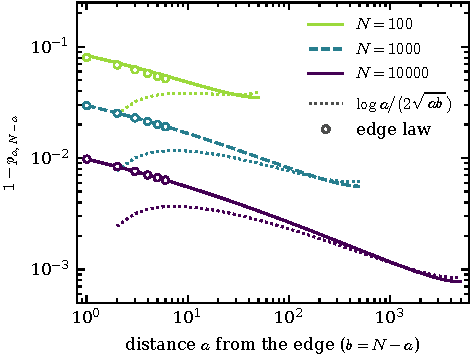
\includegraphics{figures/allbin}
\caption{The crossing $1-p_{a,N-a}$ of each bin against its distance $a$
from the nearer edge, for $N=100$, $1000$ and $10^4$. The dotted lines are the
leading law \eqref{eq:allbin-leading}, and the circles are the edge law
\eqref{eq:edge-q-expansion} for $a\le6$. The right end of each line is the
central crossing $1-p_N$.}
\label{fig:allbin}
\end{figure}

\subsection{Fixed bins and the Laguerre edge law}\label{sec:allbin-edge}

Now let $a$ be fixed and $b\to\infty$. A run of $\sR$'s away from the ends
needs 2 switches, which gives a factor $u^2$, and it can go in about $b$
places. So the right variable is $y=bu^2$. Define
\begin{equation}\label{eq:edge-polynomial}
 H_a(y)=\sum_{r=0}^{a-1}\binom{a-1}{r}\frac{y^{r+1}}{(r+1)!}
 =\frac ya L_{a-1}^{(1)}(-y),
\end{equation}
with the standard Laguerre polynomial $L_{a-1}^{(1)}$. Let $y_a$ be the
positive root of $H_a(y_a)=1$ and $c_a=\sqrt{y_a}$. Then $y_1=1$,
$y_2=\sqrt3-1$, and $y_a$ decreases strictly in $a$, by coefficient
comparison.

\begin{theorem}[fixed-edge expansion]\label{thm:edge-laguerre}
For each fixed positive integer $a$, as $b\to\infty$,
\begin{equation}\label{eq:edge-crossing-expansion}
 u_{a,b}=\frac{c_a}{\sqrt b}-\frac1b
 +\frac{\gamma_a}{b^{3/2}}+O_a(b^{-2}),
\end{equation}
where
\[
 \gamma_a=
 \frac{1+y_a+(y_a+y_a^2/2)H_a''(y_a)/H_a'(y_a)}{2c_a}.
\]
Thus the second coefficient in the odds expansion is $-1$ for every fixed
bin. For the switching probability,
\begin{equation}\label{eq:edge-q-expansion}
 1-p_{a,b}=\frac{c_a}{\sqrt b}-\frac{1+c_a^2}{b}+O_a(b^{-3/2}).
\end{equation}
\end{theorem}

In words, bin $a$ near the edge crosses at odds about $\sqrt{y_a/b}$, and the
first correction does not depend on $a$. For bin $1$ this gives
$u_{1,b}=b^{-1/2}-b^{-1}+b^{-3/2}+\dots$, the expansion of the exact root
$1/(1+\sqrt b)$ of Proposition~\ref{prop:adjacent}.

\begin{proof}
Put $\epsilon=b^{-1/2}$, $y=bu^2$ and $V_r=U_r(b)$. For $b\ge a$,
\eqref{eq:allbin-polynomial} reads
\begin{align}
 S_{a,b}(u)={}&2\sqrt{y/b}\sum_r\binom{a-1}{r}\frac{y^r}{r!}V_r\notag\\
 &+\frac yb\sum_r\binom{a-1}{r+1}\frac{y^r}{r!}V_r
 +y\sum_r\binom{a-1}{r}\frac{y^r}{(r+1)!}V_{r+1}.
 \label{eq:edge-exact-series}
\end{align}
These sums have at most $a$ terms, and with $V_r=1$ they are $H_a'(y)$,
$H_a''(y)$ and $H_a(y)$. Expanding $V_r=1-r(r+1)/(2b)+O_a(b^{-2})$ and using
$\sum_r(r+1)(r+2)\binom{a-1}{r}\frac{y^{r+1}}{(r+1)!}=y^2H_a''(y)+2yH_a'(y)$
gives, uniformly near $y=y_a$,
\begin{align}
 S_{a,b}(u)={}&H_a(y)+2\sqrt y\,H_a'(y)\epsilon\notag\\
 &+\{(y-y^2/2)H_a''(y)-yH_a'(y)\}\epsilon^2+O_a(\epsilon^3).
 \label{eq:edge-implicit-expansion}
\end{align}
With $b=\epsilon^{-2}$ the right side of \eqref{eq:edge-exact-series} is
analytic in $(\epsilon,y)$ near $(0,y_a)$, and $H_a'(y_a)>0$. So the
implicit-function theorem gives an analytic solution
$y(\epsilon)=y_a+d_1\epsilon+d_2\epsilon^2+O_a(\epsilon^3)$ of $S_{a,b}=1$,
and by the uniqueness of the crossing it is the value of $y$ at $u=u_{a,b}$.
Matching coefficients in \eqref{eq:edge-implicit-expansion} gives $d_1=-2c_a$
and $d_2=2+y_a+(y_a+y_a^2/2)H_a''(y_a)/H_a'(y_a)$. Expanding $u=\epsilon\sqrt y$
and then $u/(1+u)$ proves both expansions.
\end{proof}

For large $a$ the Laguerre root $y_a$ should obey the growing-distance law
\eqref{eq:allbin-growing-edge}. The next theorem shows this.

\begin{theorem}[matching the edge and Bessel regimes]\label{thm:edge-matching}
For every positive integer $a$ and every $x>0$,
\begin{equation}\label{eq:laguerre-bessel-bound}
 0\le1-\frac{aH_a(x^2/a)}{xI_1(2x)}\le\frac{x^2}{2a}.
\end{equation}
Consequently, with $\ell=\log a$ and $C_0=\tfrac12\log(8\pi)$, as $a\to\infty$,
\begin{align}
 2\sqrt{a y_a}
 ={}&\ell-\tfrac12\log\ell+C_0\notag\\
 &+\frac{\tfrac14\log\ell-\tfrac12C_0+3/8}{\ell}
 +O\left(\frac{(\log\ell)^2}{\ell^2}+\frac{(\log a)^2}{a}\right).
 \label{eq:edge-matching-expansion}
\end{align}
\end{theorem}

\begin{proof}
With $U_r=U_r(a)$, $aH_a(x^2/a)=x\sum_{r\ge0}U_rx^{2r+1}/(r!(r+1)!)$, so
Lemma~\ref{lem:clipped}(b) and the second identity of
Lemma~\ref{lem:clipped}(c) give \eqref{eq:laguerre-bessel-bound}. Put
$x_a=\sqrt{ay_a}$, so $aH_a(x_a^2/a)=a$, and $x_a<\log a$ for large $a$ by
\eqref{eq:laguerre-bessel-bound}. So $a\le G_0(x_a)\le a/(1-x_a^2/(2a))$, and
as in Corollary~\ref{cor:allbin-root-bound}, $x_a-x_0=O((\log a)^2/a)$, where
$G_0(x_0)=a$. So $z=2x_0$ satisfies
$z+\frac12\log z=\ell+C_0+3/(8z)+O(z^{-2})$ by \cite[Eq.~10.40.1]{dlmf}, as in
the proof of Theorem~\ref{thm:allbin-expansion} with $\eta=0$ and $A=a$, and
Lemma~\ref{lem:inversion} gives the expansion.
\end{proof}

Figure~\ref{fig:allbin} compares these laws with the exact crossings.

\subsection{The moving boundary layer}\label{sec:allbin-layer}

The crossings also give the shape of a whole row at odds $u=v_N>0$. Between
the central crossing ($v_N$ about $(\log N)/N$) and the adjacent one ($v_N$
about $N^{-1/2}$), the middle is above the endpoints and a layer of bins next
to each edge is below them. How thick is this layer? Let
\[
 \mathcal L_N=\#\{1\le k\le\lfloor N/2\rfloor:P_N(k)<P_N(0)\}.
\]

\begin{corollary}[boundary-layer width]\label{cor:boundary-layer}
Suppose that, as $N\to\infty$,
\[
 \Omega_N=\frac1{\sqrt N\,v_N}\longrightarrow\infty,
 \qquad \frac{\log\Omega_N}{Nv_N}\longrightarrow0.
\]
Then
\begin{equation}\label{eq:boundary-layer-width}
 \mathcal L_N\sim\Omega_N^2\log^2\Omega_N
 =\frac{\log^2(1/(\sqrt N\,v_N))}{Nv_N^2}.
\end{equation}
In particular, if $v_N=N^{-\gamma}$ with $1/2<\gamma<1$, then
\[
 \mathcal L_N\sim(\gamma-\tfrac12)^2N^{2\gamma-1}\log^2N.
\]
By symmetry, the total number of interior bins below the endpoint height
is $2\mathcal L_N$ for all sufficiently large $N$.
\end{corollary}

\begin{proof}
Set $d_N=\Omega_N^2\log^2\Omega_N$. Then $d_N\to\infty$ and
$d_N/N=(\log\Omega_N/(Nv_N))^2\to0$. Fix $\varepsilon\in(0,1)$ and integers
$a_\pm=(1\pm\varepsilon)d_N+O(1)$. Then $\log a_\pm\sim2\log\Omega_N$ and
$\sqrt{a_\pm(N-a_\pm)}\,v_N\sim\sqrt{1\pm\varepsilon}\,\log\Omega_N$, so
\eqref{eq:allbin-leading} gives
$u_{a_\pm,N-a_\pm}/v_N\to1/\sqrt{1\pm\varepsilon}$. Bin $k$ is below the
endpoint exactly when $v_N<u_{k,N-k}$, and $u_{k,N-k}$ decreases strictly for
$k\le N/2$ by Proposition~\ref{prop:allbin-order}. So
$a_-\le\mathcal L_N<a_+$ for large $N$, and we let $\varepsilon\downarrow0$.
Finally $\mathcal L_N=o(N)$, so the reflected intervals are disjoint.
\end{proof}
